\subsection{Валидация \texttt{NuPropagator}}

Сравнение выполнено с пакетом \texttt{nuFATE}~\cite{Vincent_2017}, реализующим аналогичный подход к расчёту прохождения нейтрино через Землю. 
Рассматривались потоки мюонных нейтрино, приходящих под различными зенитными углами в точку наблюдения, расположенную на глубине 1~км от поверхности. 
На поверхности Земли задавался степенной спектр $F_0(E) \propto E^{-2}$.  

Потоки, вычисленные с помощью \texttt{NuPropagator} и \texttt{nuFATE}, обозначим как $F_\nu^{(1)}$ и $F_\nu^{(2)}$, соответственно. 
Для количественной оценки различий введена асимметрия
\begin{equation}
\delta_{\text{asym}} = 
2\,\frac{F_\nu^{(1)}(E, x) - F_\nu^{(2)}(E, x)}
       {F_\nu^{(1)}(E, x) + F_\nu^{(2)}(E, x)}.
\end{equation}

\begin{figure}[!h]
\centering
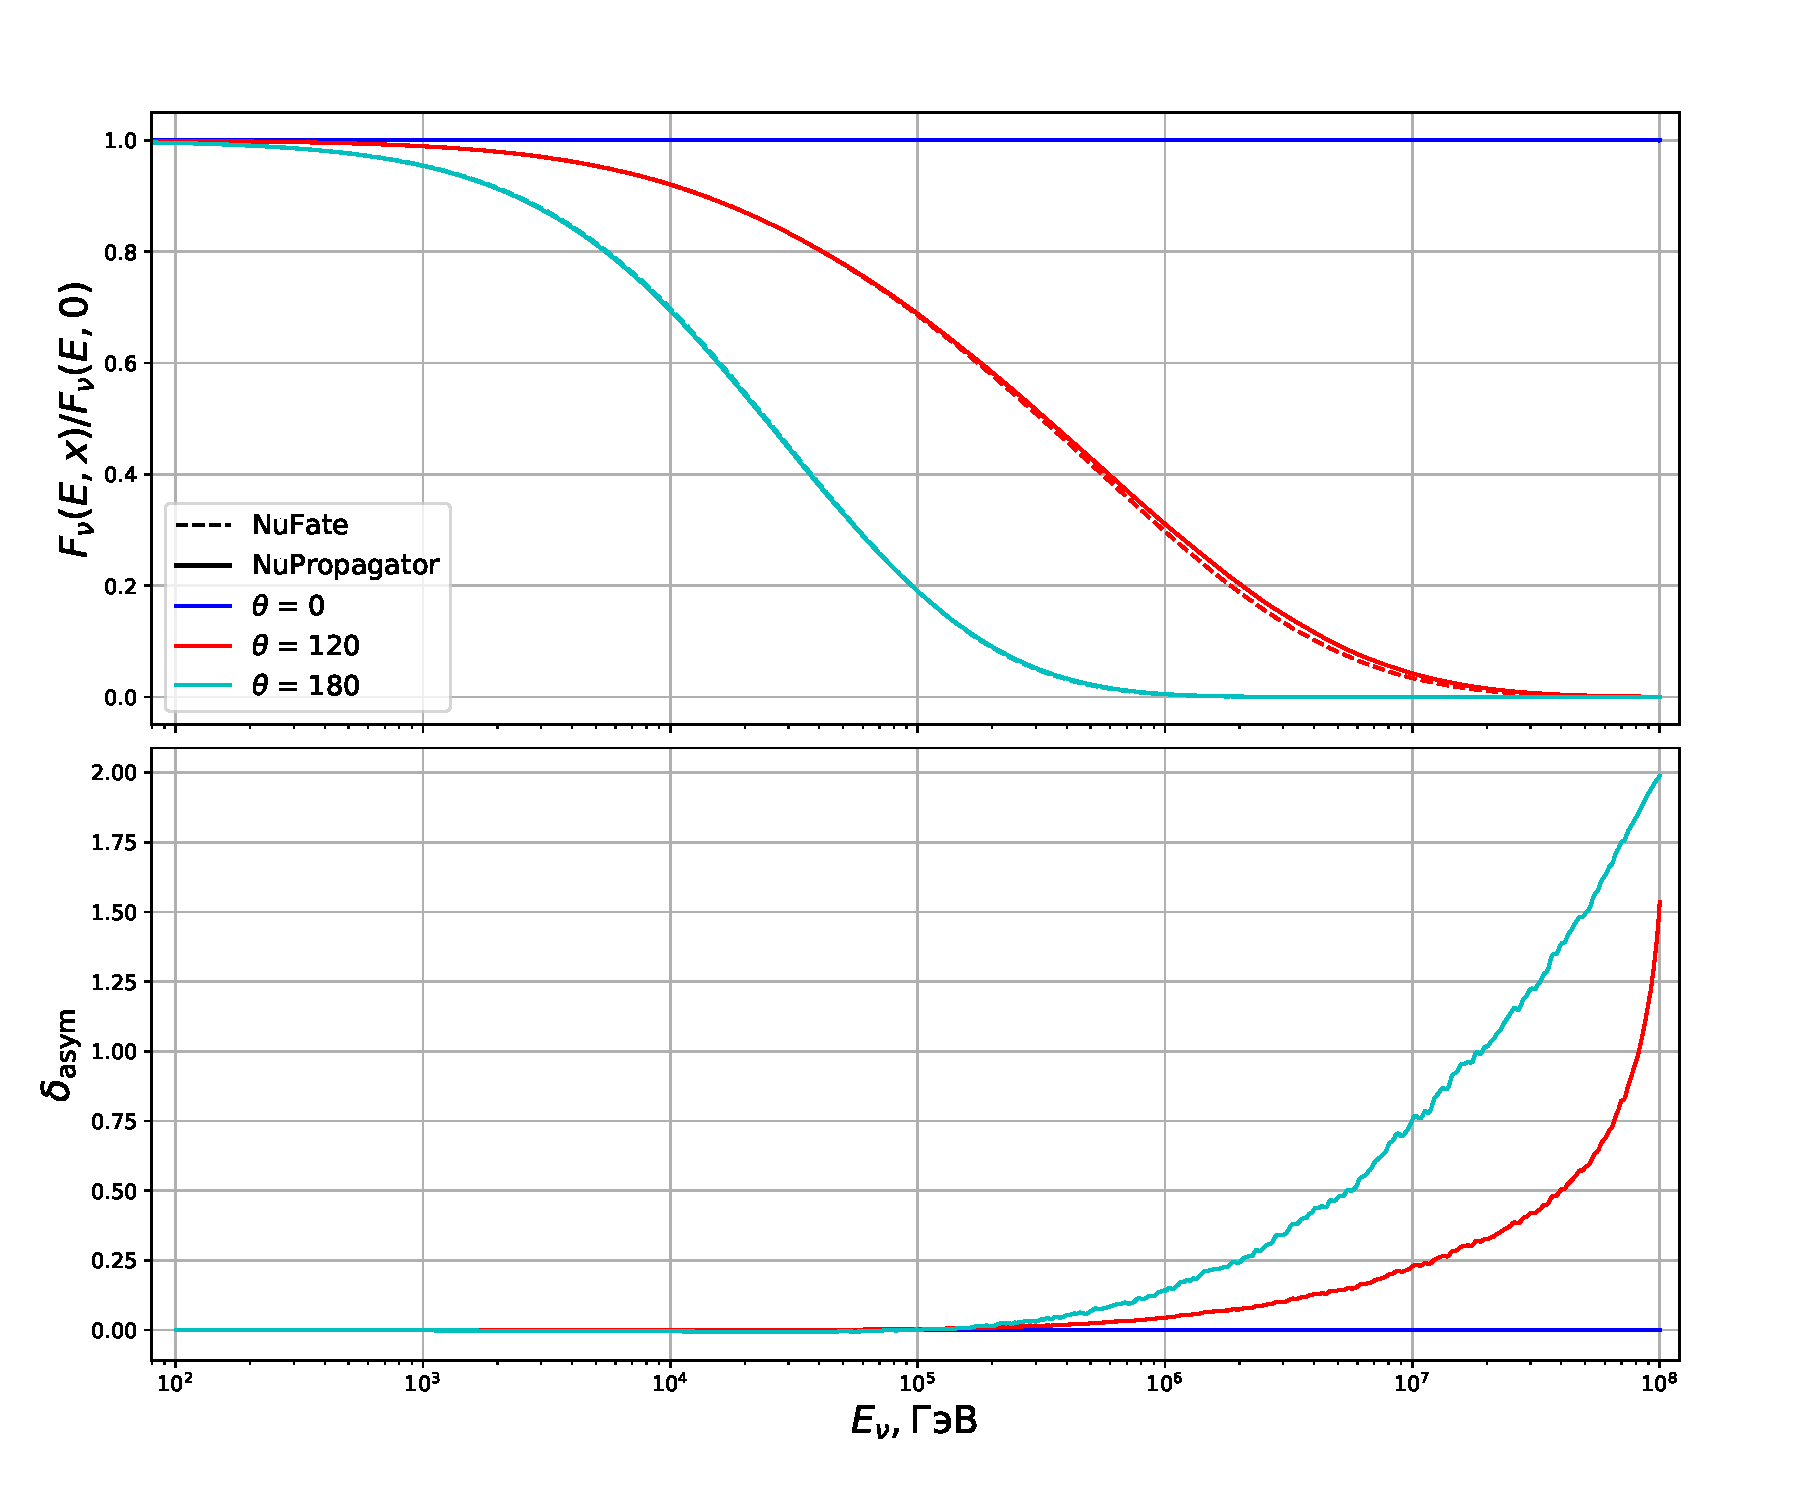
\includegraphics[width=\linewidth]{images/NuProp/compNuandNu.pdf}
\caption{Сравнение потоков нейтрино, рассчитанных с помощью \texttt{NuPropagator} и \texttt{nuFATE}, при различных зенитных углах.}
\label{fig:flux_compare}
\end{figure}

Как видно из рис.~\ref{fig:flux_compare}, оба расчёта дают близкие результаты при энергиях $E_\nu \lesssim 10^6$~ГэВ. 
Расхождения на больших энергиях обусловлены различиями в учёте регенерации потока за счёт таонных нейтрино, в моделях сечений и в численных схемах решения кинетического уравнения.
